\documentclass{article}

\usepackage{graphicx}
\usepackage{tikz}
\usepackage{tikzsymbols}
\usetikzlibrary{calc,patterns,shapes.geometric}
\pagestyle{empty}
\usepackage[margin=0pt]{geometry}
\geometry{papersize={14in,12in}}

\def\centerarc[#1](#2)(#3:#4:#5){\draw[#1] ($(#2)+({#5*cos(#3)},{#5*sin(#3)})$) arc (#3:#4:#5);}

\begin{document}
	\begin{figure}
		\centering
		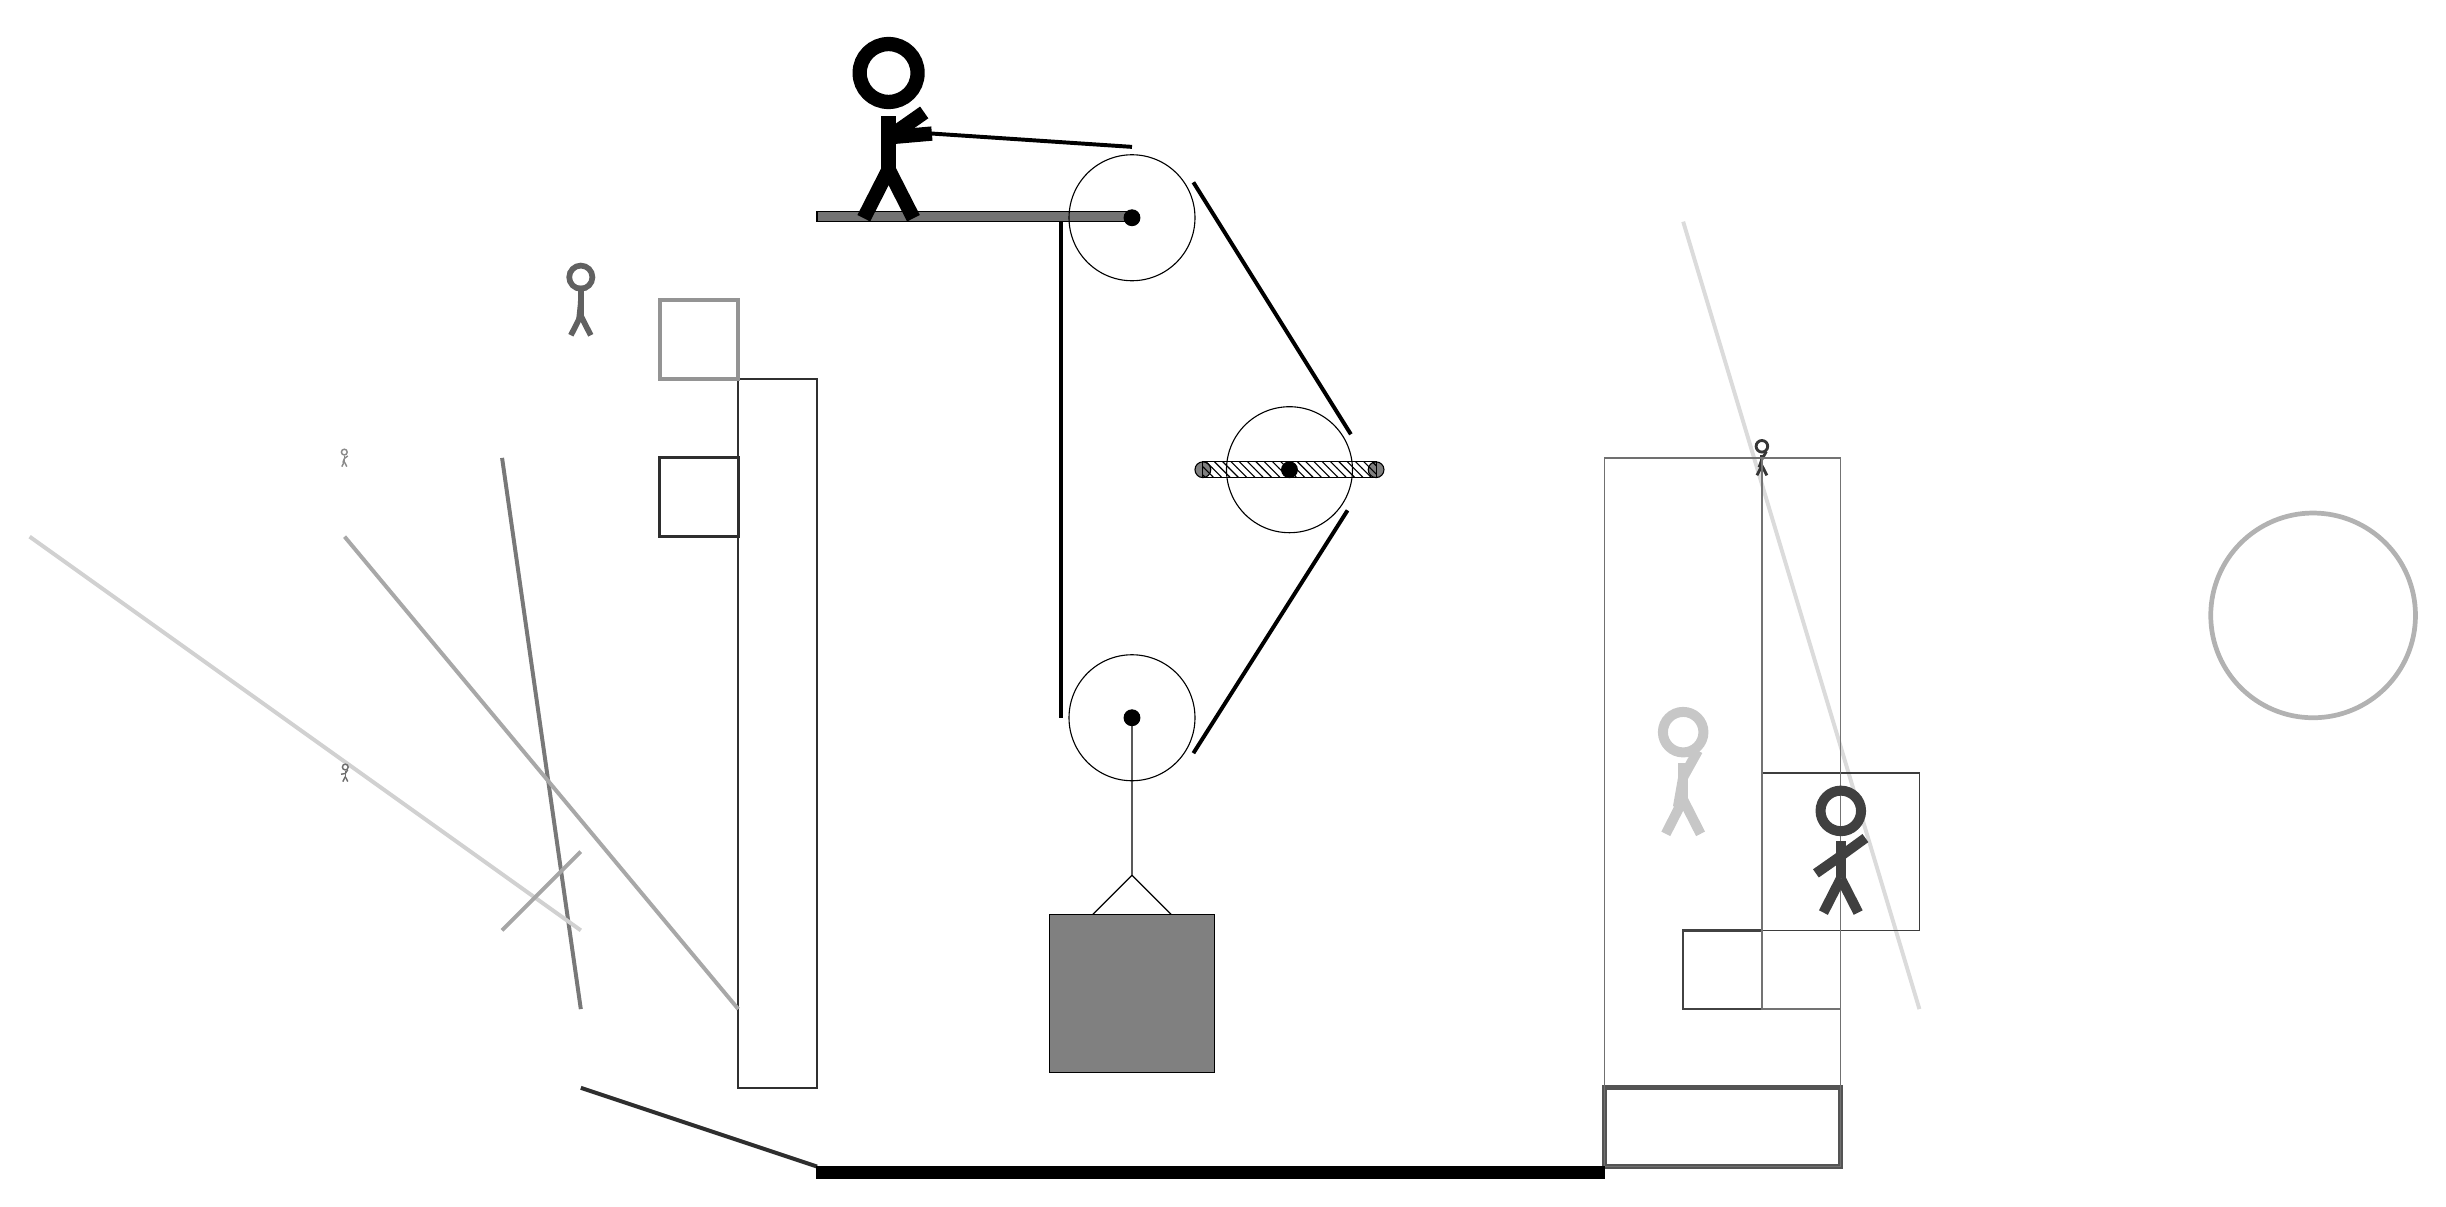
\begin{tikzpicture}
			%%%%% START %%%%%
			
			\draw[fill=black!55] (-2, 9) rectangle (2, 9.125);
			
			\draw (2, 2.7) circle (0.8);
			\draw[fill=black] (2, 2.7) circle (0.1);
			
			\draw (2, 9.05) circle (0.8);
			\draw[fill=black] (2, 9.05) circle (0.1);
			
			\draw[fill=white](4, 5.85) circle (0.8);
			\draw[fill=black] (4, 5.85) circle (0.1);
			\draw[fill=black!50] (2.9, 5.85) circle (0.1);
			\draw[fill=black!50] (5.1, 5.85) circle (0.1);
			\draw[pattern=north west lines, pattern color=black] (2.9, 5.95) rectangle (5.1, 5.75);
			
			\draw (2, 2.7) -- (2, 0.7) -- (1.5, 0.2) -- (2.5, 0.2) -- (2, 0.7);
			\draw[fill=black!50] (0.95, 0.2) rectangle (3.05, -1.8);
			
			\draw[line width=0.5mm, color=black!14](12, -1) -- (9, 9);
			
			\draw[line width=0.5mm, color=black!53](-6, 6) -- (-5, -1);
			\draw[line width=0.6mm, color=black!67] (8, -2) rectangle (11, -3);
			\draw[line width=0.3mm, color=black!81] (-3, 7) rectangle (-2, -2);
			\draw[line width=0.5mm, color=black!42] (-4, 7) rectangle (-3, 8);
			
			\node[line width=0.5mm, color=black!79] at (10, 6) {\Strichmaxerl[2][71][60]};
			
			\draw[line width=0.2mm, color=black!56] (8, -3) rectangle (11, 6);
			\draw[line width=0.5mm, color=black!18](-5, 0) -- (-12, 5);
			\draw[line width=0.3mm, color=black!74] (10, -1) rectangle (9, 0);
			\draw[line width=0.2mm, color=black!76] (10, 2) rectangle (12, 0);
			\draw[line width=0.5mm, color=black!35](-5, 1) -- (-6, 0);
			\node[line width=0.4mm, color=black!57] at (-8, 2) {\Strichmaxerl[1][10][57]};
			\draw[line width=0.5mm, color=black!82](-5, -2) -- (-2, -3);
			
			\draw[line width=0.2mm, color=black!55] (10, 6) rectangle (11, -1);
			\node[line width=0.2mm, color=black!22] at (9, 2) {\Strichmaxerl[7][80][61]};
			\draw[line width=0.4mm, color=black!82] (-4, 6) rectangle (-3, 5);
			
			\node[line width=0.2mm, color=black!62] at (-5, 8) {\Strichmaxerl[4][84][89]};
			
			\draw [line width=0.6mm, color=black!30](17, 4) circle (1.3);
			\node[line width=0.2mm, color=black!46] at (-8, 6) {\Strichmaxerl[1][71][37]};
			\draw[line width=0.5mm, color=black!34](-3, -1) -- (-8, 5);
			\node[line width=0.5mm, color=black!75] at (11, 1) {\Strichmaxerl[7][35][36]};
			
			\draw[line width=0.5mm] (1.1, 9) -- (1.1, 2.7);
			\centerarc[line width=0.5mm](2, 2.7)(180:330:0.9);
			\draw[line width=0.5mm](2.7794, 2.25) -- (4.7373, 5.3338);
			\centerarc[line width=0.5mm](4, 5.85)(390:325:0.9);
			\draw[line width=0.5mm](4.7794, 6.3) -- (2.7794, 9.5);
			\centerarc[line width=0.5mm](2, 9.05)(30:90:0.9);
			\draw[line width=0.5mm](2, 9.95) -- (-1, 10.15);
			
			\node at (-1, 10.15) {\Strichmaxerl[10][-175][35]};
			
			\draw[fill=black] (-2, -3) rectangle (8, -3.15);
			
			%%%%% END %%%%%
		\end{tikzpicture}
	\end{figure}	
\end{document}